\documentclass[conference]{IEEEtran}
\IEEEoverridecommandlockouts

\usepackage{cite}
\usepackage{amsmath,amssymb,amsfonts}
\usepackage{graphicx}
\usepackage{textcomp}
\usepackage{xcolor}
\usepackage{booktabs}
\usepackage{multirow}
\usepackage{array}
\usepackage{url}
\usepackage[ruled,vlined,linesnumbered]{algorithm2e}
\usepackage{tikz}
\usetikzlibrary{positioning,arrows.meta,fit,backgrounds}
\SetAlFnt{\small}
\SetKwInOut{Input}{Input}
\SetKwInOut{Output}{Output}
\SetKw{KwSkip}{skip}

\graphicspath{{figures/}}

% Marks text that still waits for a saved result. Remove the macro calls
% once the numbers are filled in from results/; the paper must not be
% submitted while any \pending remains.
\newcommand{\pending}[1]{\textcolor{red}{[PENDING: #1]}}

% While figures and generated tables are missing (e.g. a first upload to
% Overleaf), show a red placeholder instead of stopping the build.
\newcommand{\safefig}[2][\columnwidth]{\IfFileExists{figures/#2.pdf}{\includegraphics[width=#1]{#2}}{\IfFileExists{figures/#2.png}{\includegraphics[width=#1]{#2}}{\fbox{\parbox{0.9\linewidth}{\centering\pending{figure \detokenize{#2}}}}}}}
\newcommand{\safetable}[1]{\IfFileExists{tables/#1.tex}{\input{tables/#1}}{\pending{table \detokenize{#1}, generated by scripts/make\_paper\_tables.py}}}

% allow two full-width floats (Table I and Fig. 1) at the top of one page
\renewcommand{\dbltopfraction}{0.85}
\begin{document}

\title{Does Robust Adaptive Thresholding Help LSTM Autoencoder Anomaly Detection? A Leakage-Free Evaluation on NAB}

\author{\IEEEauthorblockN{Zain Hassan}
\IEEEauthorblockA{\textit{Dept. of Artificial Intelligence and Data Science} \\
\textit{National University of Computer and Emerging Sciences}\\
Islamabad, Pakistan \\
hassanmangat03217@gmail.com}
}

\maketitle

\begin{abstract}
We hold one LSTM autoencoder fixed and change only the rule that turns its reconstruction error into an alarm. The base rule, taken from a recent AIOps pipeline, thresholds the mean absolute error of each 30-step window at the mean plus three standard deviations of the training errors. Our proposed rule (P1) recomputes the median plus $\lambda$ scaled median absolute deviations (MAD) over the last $w$ errors. Eight rules run on the same errors from the Numenta Anomaly Benchmark (NAB): the base rule, percentile and mean plus $k\sigma$ baselines, a static median plus MAD rule, an extreme value threshold, the rolling mean plus $3\sigma$ rule of RePAD2 with fixed and tuned multipliers, and P1. Each series is split 60/20/20 in time, every parameter is tuned on validation data only, and 18 test series are scored once per seed (15, 42 and 123) under tests fixed before any threshold result existed. The base rule caught 24 of the 25 test windows but flagged 18.9\% of normal points. Rolling thresholds cut that rate to 1.8\% (RePAD2 rule, $w = 400$) and 3.5\% (P1, $w = 50$, $\lambda = 6$). P1 also missed 6.7 windows on average, and its composite F1 fell to 0.544 against 0.733 for the base rule (Wilcoxon $p = 0.035$). No confirmatory hypothesis held. Recomputing the threshold from recent errors removes most false alarms; replacing the mean and standard deviation with the median and MAD does not add to that gain.
\end{abstract}

\begin{IEEEkeywords}
anomaly detection, LSTM autoencoder, dynamic threshold, median absolute deviation, AIOps, Numenta Anomaly Benchmark
\end{IEEEkeywords}

%=====================================================================
\section{Introduction}
%=====================================================================

An LSTM autoencoder (LSTM-AE) monitor has two stages. The network reconstructs a sliding window of a metric such as CPU load or request count, and a threshold rule decides which reconstruction errors become alarms. The second stage sets the false-alarm rate an operator lives with, yet comparisons usually change the model and the threshold together, so the threshold's own effect stays hidden. Surveys of microservice anomaly detection \cite{soldani2022} and of deep time-series detectors \cite{darban2024} map a field organised around model families.

Ahmad \cite{ahmad2026} describes one such AIOps pipeline and fixes the threshold at $\mu + 3\sigma$ of the training errors, once, after training. The preprint calls this rule dynamic and reports no detection metrics. Our project proposal predicted a specific weakness: large training errors raise both $\mu$ and $\sigma$, the threshold widens, and later anomalies pass under it. The median and the MAD have a breakdown point of 50\%, against 0\% for the mean, so a minority of extreme errors cannot move them. We therefore recompute a median plus $\lambda\cdot$MAD threshold over the last $w$ errors (rule P1) and test it against the base rule and six alternatives on identical reconstruction errors.

The prediction failed, and in an unexpected direction. Our contributions are:
\begin{itemize}
\item a controlled comparison of eight threshold rules on one shared LSTM-AE, including the rolling rule of RePAD2 \cite{lee2023repad2} and the extreme value rule of Yu et al. \cite{yu2024evt};
\item a leakage-free protocol with label-free training, validation-only tuning, equal tuning budgets for Gaussian and robust rules, and one test scoring;
\item a negative result with its causes: P1 trails the rolling mean rule, and four test streams expose where its short robust buffer fails;
\item a public code base with a scorer port validated against NAB and a script that traces every number in this paper to a result file.
\end{itemize}

The research questions follow the project proposal:
\begin{enumerate}
\item[RQ1] How do the static percentile, mean plus $k\sigma$ and base $\mu + 3\sigma$ rules perform on NAB?
\item[RQ2] How does P1 compare with these baselines on F1 and NAB score?
\item[RQ3] How far does P1 cut false alarms where normal variability rises?
\item[RQ4] Which NAB categories gain most from P1 over the baselines?
\end{enumerate}

%=====================================================================
\section{Related Work}
%=====================================================================

\subsection{Deep anomaly detection and its evaluation}
Reconstruction-based models such as the LSTM-AE form one of the main families in the taxonomy of Darban et al. \cite{darban2024}, next to forecasting-based models. How these models are scored decides how they rank. Kim et al. \cite{kim2022} show that point adjustment inflates F1 until an untrained model looks competitive, and Paparrizos et al. \cite{paparrizos2022} show that the evaluation measure alone can bias a comparison; Garg et al. \cite{garg2022} answer with the composite F-score, which pairs point-wise precision with event-wise recall, and find dynamic scoring functions ahead of static ones. Results also vary widely across algorithms and datasets in the evaluation of Schmidl et al. \cite{schmidl2022}, which covers 71 algorithms on 967 time series. Wu and Keogh \cite{wu2023} question the benchmarks themselves, NAB included, citing trivial anomalies, unrealistic anomaly density, mislabelled ground truth and run-to-failure bias. These warnings fix our metric choices (Section~\ref{sec:metrics}) and several of our limitations.

\subsection{Thresholds for reconstruction and prediction errors}
Threshold rules for LSTM detectors differ along two axes: whether the statistic is recomputed over time, and whether labels are needed (Table~\ref{tab:related}). Ahmad \cite{ahmad2026} and Yu et al. \cite{yu2024evt} both fit a static threshold to LSTM-AE training errors, the first as $\mu + 3\sigma$ and the second as a generalized Pareto tail quantile chosen by an unsupervised criterion, which on spacecraft telemetry raised precision from 85.8\% under the $3\sigma$ rule to 92.4\%. RePAD2 \cite{lee2023repad2} instead recomputes the mean plus three standard deviations over the most recent $W$ errors of a small LSTM predictor, while Jeon et al. \cite{jeon2023} place the threshold between the largest normal and the smallest anomalous error and therefore need labelled anomalies. None of these studies compares static with rolling rules, or Gaussian with robust statistics, on the same model errors. Only two use NAB, on one series (Ahmad) and two series (RePAD2).

\begin{table*}[t]
\centering
\caption{Closest related work on thresholds for LSTM-based detectors.}
\label{tab:related}
\footnotesize
\setlength{\tabcolsep}{4pt}
\begin{tabular}{@{}>{\raggedright\arraybackslash}p{2.0cm}>{\raggedright\arraybackslash}p{2.5cm}>{\raggedright\arraybackslash}p{4.1cm}>{\raggedright\arraybackslash}p{2.9cm}>{\raggedright\arraybackslash}p{1.3cm}>{\raggedright\arraybackslash}p{3.6cm}@{}}
\toprule
Study & Model / score & Threshold rule & Data & Labels for threshold & Limitation for our question \\
\midrule
Ahmad \cite{ahmad2026} & LSTM-AE, window MAE & $\mu + 3\sigma$ of training errors, fixed after training & NAB EC2 CPU (one series) & No & Preprint; no quantitative metrics; ``dynamic'' rule is static \\
Lee \& Lin \cite{lee2023repad2} & LSTM predictor, AARE & Mean $+ 3\sigma$ over the last $W$ scores & Two NAB series, concatenated ten times & No & Gaussian statistics only; $W \geq 1440$ \\
Yu et al. \cite{yu2024evt} & LSTM-AE, squared error & GPD tail quantile (POT), $q$ by an unsupervised criterion; dynamic update & Tennessee Eastman, spacecraft telemetry & No & Dynamic update ambiguous as printed; not on NAB \\
Jeon et al. \cite{jeon2023} & LSTM-AE & Ratio $\alpha$ between max normal and min anomalous error & Pump sensors (Kaggle) & Yes & Needs labelled anomalies \\
This work & LSTM-AE \cite{ahmad2026}, window MAE & Eight rules incl. rolling median + $\lambda\cdot$MAD & NAB, 18 test series & Validation only & Single model and benchmark \\
\bottomrule
\end{tabular}
\end{table*}

\subsection{Research gap}
We found no study that tests a rolling median plus MAD threshold on LSTM-AE errors while keeping tuning away from the test data. Controlled comparisons that hold the model fixed and vary only the threshold, the one setting that judges a threshold rule on its own, are rare.

%=====================================================================
\section{Data}
%=====================================================================

\subsection{The Numenta Anomaly Benchmark}
We use NAB \cite{nab2024}, pinned at commit \texttt{ea702d7}. It contains 58 univariate series in seven categories (artificial with and without anomalies, AWS CloudWatch, ad exchange, known-cause incidents, traffic and Twitter volume), 365,558 points in total, with 116 labelled anomaly windows that cover 9.16\% of all points. NAB labels windows, not single points, and its scoring rewards early detection inside a window.

\subsection{Exploratory analysis and file selection}
Every series is split chronologically into 60\% training, 20\% validation and 20\% test. Of the 116 windows, 65 touch the training part, 31 the validation part and 25 the test part; five cross a boundary. Only 18 series have a window in their test part, so these 18 series, all real data, form the evaluation set and contain all 25 test windows (Fig.~\ref{fig:split}). The tuning set consists of the 24 real series with a window in their validation part. We left out the artificial series, so that tuning matches the all-real evaluation set, and \texttt{grok\_asg\_anomaly}, whose window runs from validation into test. Six series are in both sets, which is safe because their validation and test parts do not overlap in time. The 18 tuning-only series have anomaly-free test parts, which we use to measure false alarms on clean data. Altogether 36 series need a model.

Training uses no labels, so anomalies reach the training data: 38 of the 52 labelled series have labelled points in their training part, 8.48\% of all training points (median 8.33\% per series, maximum 16.91\%). A deployed detector faces the same contamination, and it hits all threshold rules equally. The analysis also found 49 duplicate timestamps in 8 series and irregular sampling in 25 series, with 27,625 missing steps in total.

\begin{figure*}[t]
\centering
\safefig[\textwidth]{fig1_windows_vs_split}
\caption{Position of every NAB anomaly window relative to the 60/20/20 split. The 18 series with a window in the test part (bold, coloured by NAB category) form the evaluation set; series in grey have no test window and cannot be evaluated.}
\label{fig:split}
\end{figure*}

\subsection{Preprocessing and leakage prevention}
Four rules keep labels and test data out of training and tuning:
\begin{enumerate}
\item \emph{Scaling.} Min--max scaling to $[0,1]$ is fitted on the training part of each series only.
\item \emph{No label filtering.} The model and all static thresholds see every training point; labels serve only validation tuning and test scoring.
\item \emph{Gaps and duplicates.} Series are not resampled, because NAB scores rows and filling gaps would move its window boundaries; a window of 30 rows therefore covers different lengths of time in irregular series. Duplicate timestamps are kept, and window edges map to the first occurrence, as in the official scorer.
\item \emph{Single test scoring.} The test parts are scored once, with parameters chosen on validation data.
\end{enumerate}

%=====================================================================
\section{Method}
%=====================================================================

\begin{figure*}[t]
\centering
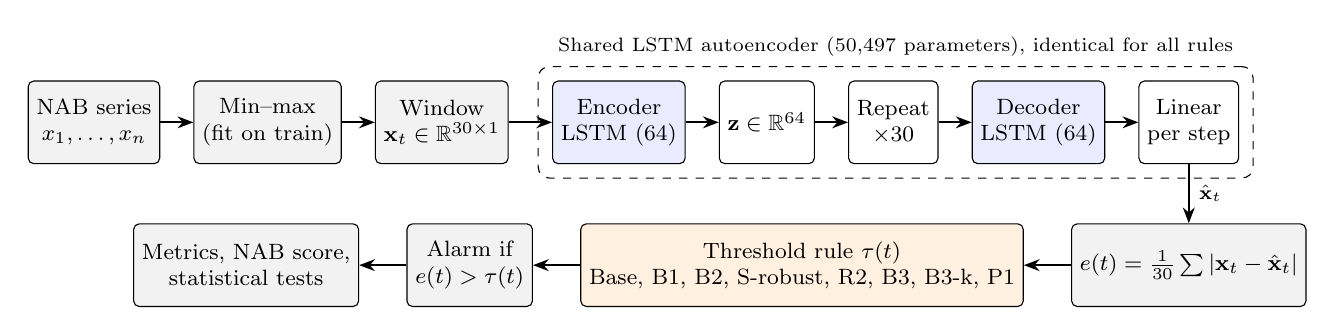
\begin{tikzpicture}[
  font=\footnotesize,
  blk/.style={draw, rounded corners=2pt, align=center, minimum height=1.05cm, inner sep=3pt, fill=white},
  lstm/.style={blk, fill=blue!8, minimum width=1.6cm},
  data/.style={blk, fill=gray!10},
  thr/.style={blk, fill=orange!12},
  arr/.style={-{Stealth[length=2mm]}, thick},
  node distance=0.42cm]
\node[data] (raw) {NAB series\\$x_1,\dots,x_n$};
\node[data, right=of raw] (scale) {Min--max\\(fit on train)};
\node[data, right=of scale] (win) {Window\\$\mathbf{x}_t \in \mathbb{R}^{30\times 1}$};
\node[lstm, right=0.55cm of win] (enc) {Encoder\\LSTM (64)};
\node[blk, right=of enc, minimum width=1.1cm] (z) {$\mathbf{z}\in\mathbb{R}^{64}$};
\node[blk, right=of z] (rep) {Repeat\\$\times 30$};
\node[lstm, right=of rep] (dec) {Decoder\\LSTM (64)};
\node[blk, right=of dec] (out) {Linear\\per step};
\node[data, below=0.75cm of out] (err) {$e(t)=\frac{1}{30}\sum |\mathbf{x}_t-\hat{\mathbf{x}}_t|$};
\node[thr, left=0.6cm of err, minimum width=4.6cm] (rule) {Threshold rule $\tau(t)$\\Base, B1, B2, S-robust, R2, B3, B3-k, P1};
\node[data, left=0.6cm of rule] (alarm) {Alarm if\\$e(t) > \tau(t)$};
\node[data, left=0.6cm of alarm] (eval) {Metrics, NAB score,\\statistical tests};
\draw[arr] (raw) -- (scale); \draw[arr] (scale) -- (win); \draw[arr] (win) -- (enc);
\draw[arr] (enc) -- (z); \draw[arr] (z) -- (rep); \draw[arr] (rep) -- (dec); \draw[arr] (dec) -- (out);
\draw[arr] (out) -- node[right, font=\scriptsize]{$\hat{\mathbf{x}}_t$} (err);
\draw[arr] (err) -- (rule); \draw[arr] (rule) -- (alarm); \draw[arr] (alarm) -- (eval);
\begin{scope}[on background layer]
\node[draw, dashed, rounded corners, fit=(enc)(z)(rep)(dec)(out), inner sep=5pt,
      label={[font=\scriptsize]above:Shared LSTM autoencoder (50,497 parameters), identical for all rules}] {};
\end{scope}
\end{tikzpicture}
\caption{Pipeline. One LSTM autoencoder, following the base paper \cite{ahmad2026}, produces the reconstruction error $e(t)$ for every series; the compared methods differ only in the threshold rule.}
\label{fig:pipeline}
\end{figure*}

\subsection{Shared LSTM autoencoder}
All methods share one model that follows the base paper \cite{ahmad2026} (Fig.~\ref{fig:pipeline}): an LSTM encoder with 64 units, its last hidden state repeated over the window, an LSTM decoder with 64 units and a linear output per step, 50,497 parameters in total. Windows have $T = 30$ steps. The model is trained with Adam (learning rate $10^{-3}$, batch size 32) on the mean squared error for up to 50 epochs, with early stopping (patience 5) on the last 10\% of the training part. The anomaly score $e(t)$ is the mean absolute error of the window that ends at $t$, so scores are causal. We use PyTorch on CPU instead of the paper's Keras; the architecture is unchanged. Each of the 36 series is trained with three seeds (15, 42, 123), giving 108 error series.

\subsection{Threshold rules}
Every rule raises an alarm when $e(t)$ exceeds its threshold $\tau(t)$. Static rules compute one $\tau$ from the training errors $E_{\mathrm{tr}}$; rolling rules compute $\tau(t)$ from a buffer $B_t$ of the $w$ errors before $t$, over one continuous stream.
\begin{itemize}
\item \textbf{Base} \cite{ahmad2026}: $\tau = \mathrm{mean}(E_{\mathrm{tr}}) + 3\,\mathrm{sd}(E_{\mathrm{tr}})$, untuned.
\item \textbf{B1}: $\tau$ = the $p$-th percentile of $E_{\mathrm{tr}}$, $p$ tuned.
\item \textbf{B2}: $\tau = \mathrm{mean}(E_{\mathrm{tr}}) + k\,\mathrm{sd}(E_{\mathrm{tr}})$, $k$ tuned.
\item \textbf{S-robust}: $\tau = \mathrm{median}(E_{\mathrm{tr}}) + \lambda\,\mathrm{MAD}(E_{\mathrm{tr}})$, $\lambda$ tuned.
\item \textbf{R2} \cite{yu2024evt}: $\tau$ = a generalized Pareto tail quantile of $E_{\mathrm{tr}}$, untuned.
\item \textbf{B3} \cite{lee2023repad2}: $\tau(t) = \mathrm{mean}(B_t) + 3\,\mathrm{sd}(B_t)$, $w$ tuned.
\item \textbf{B3-k}: $\tau(t) = \mathrm{mean}(B_t) + k\,\mathrm{sd}(B_t)$, $k$ and $w$ tuned.
\item \textbf{P1 (proposed)}: $\tau(t)$ from \eqref{eq:p1}, $\lambda$, $w$ and memory tuned.
\end{itemize}
R2 fits the generalized Pareto distribution by maximum likelihood to the excesses over the 98\% quantile of $E_{\mathrm{tr}}$ and picks the tail probability $q \in [10^{-5}, 10^{-3}]$ with the paper's unsupervised criterion on training errors. We reproduce only this fully specified static part: as printed, the dynamic update multiplies the threshold by a factor in $[1, 2)$, so it can only grow, and its update frequency is not given. The RePAD2 window lengths exceed many NAB series, so B3 tunes $w$; B3-k also tunes $k$, which gives the Gaussian and robust rolling rules the same tuning budget. P1 computes
\begin{equation}
\tau(t) = m_t + \lambda \max\!\big(c\,\mathrm{med}|B_t - m_t|,\, \phi\big),\ \ m_t = \mathrm{med}\,B_t,
\label{eq:p1}
\end{equation}
where $\mathrm{med}$ is the median and the MAD scale $c = 1.4826$ makes $\lambda = 3$ match $3\sigma$ for Gaussian data. Rolling rules share the scale floor $\phi$, $0.1$ times the scaled MAD of $E_{\mathrm{tr}}$ (falling back to $0.1\,\mathrm{sd}$, then $10^{-6}$), so flat stretches do not trigger alarms on tiny changes. With \emph{plain} memory every error enters $B_t$. With \emph{gated} memory an error that raised an alarm stays out of $B_t$, so an anomaly cannot raise the bar it is judged by; an alarm run longer than $w$ is accepted as a new normal. B2 versus S-robust and B3-k versus P1 form the two equal-budget comparisons of Gaussian and robust statistics. Algorithm~\ref{alg:p1} gives P1 in full.

\begin{algorithm}[t]
\caption{Proposed rolling median + MAD threshold (P1)}
\label{alg:p1}
\Input{errors $e(1{:}n)$, first scored index $f$; window $w$; multiplier $\lambda$; memory $\in\{\text{plain},\text{gated}\}$; floor $\phi$}
\Output{alarms $a(1{:}n)$, thresholds $\tau(1{:}n)$}
$B \leftarrow e(f{:}f{+}w{-}1)$; \quad $R \leftarrow \emptyset$ \tcp*{buffer, run}
\For{$t \leftarrow f+w$ \KwTo $n$}{
  \lIf{memory $=$ plain}{$B \leftarrow e(t{-}w{:}t{-}1)$}
  $m \leftarrow \mathrm{median}(B)$; \quad $s \leftarrow 1.4826\cdot\mathrm{median}(|B-m|)$\;
  $\tau(t) \leftarrow m + \lambda \cdot \max(s, \phi)$\;
  \eIf{$e(t) > \tau(t)$}{
    $a(t) \leftarrow 1$\;
    \If{memory $=$ gated}{
      append $e(t)$ to $R$ \tcp*{kept out of $B$}
      \If(\tcp*[f]{new normal}){$|R| > w$}{$B \leftarrow$ last $w$ values of $R$; \quad $R \leftarrow \emptyset$\;}
    }
  }{
    $a(t) \leftarrow 0$\;
    \lIf{memory $=$ gated}{$R \leftarrow \emptyset$; replace the oldest value of $B$ by $e(t)$}
  }
}
\Return{$a$, $\tau$}
\end{algorithm}


\subsection{Tuning}
Parameters are chosen on the validation parts of the 24 tuning series over all three seeds, by mean composite F1, with ties broken by NAB score and then by alarm rate. The grids are $p \in \{90, 95, 97, 98, 99, 99.5, 99.9\}$, $k_{\mathrm{B2}} \in \{1, 1.5, 2, 2.5, 3, 4, 5, 6, 8\}$, $\lambda$ and $k_{\mathrm{B3\text{-}k}} \in \{2, 3, 4, 5, 6, 8, 10, 12, 15, 20\}$, $w \in \{50, 100, 200, 400\}$, and memory $\in$ \{plain, gated\}. One parameter set per method is used for all seeds. In total 152 candidates were scored on 72 validation series (10,944 rows). Algorithm~\ref{alg:protocol} summarises the procedure; test labels are never used before the final step.

\begin{algorithm}[t]
\caption{Leakage-free tuning and single test scoring}
\label{alg:protocol}
\Input{error series $E_{f,s}$ for series $f$ and seed $s$; tuning set $\mathcal{F}_{\mathrm{tun}}$ (24); evaluation set $\mathcal{F}_{\mathrm{eval}}$ (18); seeds $\mathcal{S}=\{15,42,123\}$; rules $\mathcal{M}$ with grids $\Theta_m$}
\Output{selected $\theta^\ast_m$ and test metrics for every rule $m$}
\ForEach{$m \in \mathcal{M}$}{
  \ForEach{$\theta \in \Theta_m$}{
    \ForEach{$f \in \mathcal{F}_{\mathrm{tun}},\ s \in \mathcal{S}$}{
      $a \leftarrow$ \textsc{Alarms}$_m(E_{f,s};\theta)$ \tcp*{whole stream}
      $c_{f,s}(\theta) \leftarrow$ composite F1 of $a$ on the validation part of $f$\;
    }
    $\bar c(\theta) \leftarrow$ mean of $c_{f,s}(\theta)$ over the 72 series\;
  }
  $\theta^\ast_m \leftarrow \arg\max_\theta \bar c(\theta)$; ties: higher NAB, then lower alarm rate\;
}
\ForEach{$m \in \mathcal{M},\ f \in \mathcal{F}_{\mathrm{eval}},\ s \in \mathcal{S}$}{
  score \textsc{Alarms}$_m(E_{f,s};\theta^\ast_m)$ \emph{once} on the test part of $f$\;
}
\end{algorithm}


%=====================================================================
\section{Experimental Design}
%=====================================================================

\subsection{Metrics}
\label{sec:metrics}
Point precision, recall and F1 count every point inside a window as positive, without point adjustment \cite{kim2022}. Event recall is the share of windows with at least one alarm, and composite F1 is the harmonic mean of point precision and event recall \cite{garg2022}. The false-positive rate (FPR) is computed over normal points. The high-variance FPR is the FPR over normal points whose 50-step rolling standard deviation exceeds the 75th percentile of that quantity in the training part; it targets RQ3. On the clean test parts we report the FPR and false alarms per 1,000 points. The NAB score comes from a port of the official scorer, which we validated against NAB's published results for three shipped detectors and three scoring profiles, with the null detector as the normalisation baseline: per-file raw scores agreed within $5.0\times10^{-12}$ and normalised scores within $1.9\times10^{-11}$. On the test parts we count every alarm step, clip windows to the segment and use no probationary period, so our NAB numbers are not comparable with the NAB leaderboard. ROC-AUC and PR-AUC on the raw errors describe the model itself and are identical for all rules. Detection delay is the number of steps from the start of a detected window to its first alarm, divided by the window length.

\subsection{Statistical protocol}
Each test series is one unit, with metrics averaged over the three seeds first ($n = 18$; $n = 17$ for high-variance FPR, which is undefined for one series that has no normal test point above the variance cut). Comparisons use the paired two-sided Wilcoxon signed-rank test at $\alpha = 0.05$, together with the mean difference, a bootstrap 95\% confidence interval and the count of wins and losses. The primary comparison is P1 against Base; P1 against every other rule is secondary and Holm-corrected within each metric. The tuning objective, the grids, B3-k and these tests were committed to the repository before any threshold result was computed. The proposal, written in October 2026 before any experiment, fixed three hypotheses:
\begin{enumerate}
\item[H1] P1 achieves a higher F1 than the baseline on at least 70\% of series.
\item[H2] P1 lowers the high-variance FPR by at least 15\% under a paired $t$-test.
\item[H3] P1 gains more on AWS CloudWatch series than on any other category.
\end{enumerate}

Experiments ran on a laptop (Intel Core i5-13500H, 15.7 GB RAM) with Python 3.12.4 and PyTorch 2.14.1 on CPU, which makes runs deterministic for a given seed. The 108 training runs took 47.5 minutes in total; tuning and test scoring took under three minutes.

%=====================================================================
\section{Results}
%=====================================================================

\subsection{Model training}
All 108 runs finished. Training stopped after 6 to 50 epochs (median 20), and ten runs reached the 50-epoch cap. Five runs had their best epoch at 1 or 2; the protocol keeps every run alike, so they stayed in. On the test parts the model reached a ROC-AUC of $0.633 \pm 0.003$ and a PR-AUC of $0.497 \pm 0.011$ (mean $\pm$ sd over seeds), a moderate ceiling on what any threshold can achieve.

\subsection{Tuning}
Validation selected $p = 90$ for B1, $k = 2.5$ for B2, $\lambda = 5$ for S-robust, $w = 400$ for B3, $k = 3$ and $w = 400$ for B3-k, and $\lambda = 6$, $w = 50$ with plain memory for P1. B3-k landed on $k = 3$, which makes it identical to B3 on the test data and reduces the equal-budget rolling comparison to B3 versus P1. Gated memory never won on validation. Four selections lie on a grid edge (B1, B3, B3-k and P1); Section~\ref{sec:explore} extends those grids. R2 took its unsupervised criterion path for 104 of the 108 error series and never needed its fallback.

\subsection{Test performance (RQ1, RQ2)}
Base caught 24 of the 25 test windows, and its weakness lies in the FPR column of Table~\ref{tab:test}. Every static rule compares test errors with a statistic of training errors, and test errors run higher than training errors (Section~\ref{sec:drift}); tuning $p$, $k$ or $\lambda$ shifts that fixed bar but cannot follow the drift. Rolling rules re-estimate the bar from the last $w$ errors, which cut the FPR to about a tenth (B3) and a fifth (P1) of the base value. P1 bought its low FPR with recall. With $w = 50$ and $\lambda = 6$, any anomaly that unfolds over tens of steps raises its own threshold, so P1's event recall dropped to 0.769 and its composite F1 to 0.544. Point F1 reverses the ranking because it credits every labelled point: B1 alarms on long stretches and scores 0.407, while the rolling rules fire in short bursts at the onset of an error rise and recover fewer points.

\begin{table*}[t]
\centering
\caption{Test results on 18 evaluation series (mean $\pm$ sd over three seeds of the across-series mean). Clean FA/1k: false alarms per thousand points on the 18 anomaly-free test parts. Generated from \texttt{results/phase3/test\_summary.csv}.}
\label{tab:test}
\safetable{test_summary}
\end{table*}

\subsection{NAB cost profiles}
The order B3, P1, Base holds under all three NAB cost profiles (corpus scores, every alarm step): $-28.7$, $-113.6$ and $-370.2$ under the standard profile, $-138.1$, $-294.4$ and $-829.5$ under reward-low-FP, and $10.2$, $-51.3$ and $-214.8$ under reward-low-FN. Doubling the false-positive weight from 0.11 to 0.22 widens Base's deficit to B3 far more than doubling the miss weight does, because Base raises roughly ten false alarms on normal test points for every one of B3's.

\subsection{Hypothesis tests (RQ2, RQ3)}
Table~\ref{tab:tests} lists the confirmatory tests of P1 against Base. The composite F1 deficit is significant, with a confidence interval that excludes zero, while the drop in high-variance FPR ($n = 17$) misses significance at $p = 0.109$ and the clean-stream FPR and every-step NAB differences are not significant. After Holm correction, P1 was worse than B3 on composite F1, clean-stream FPR and NAB, and worse than R2 on the clean-stream measures; it beat B1 on high-variance FPR and NAB. Fig.~\ref{fig:paired} shows that the deficit is broad rather than driven by one series: P1 lost on 13 of 18 series against both Base and B3.

\begin{table}[t]
\centering
\caption{Confirmatory tests, P1 against Base (paired Wilcoxon, $n$ series). Generated from \texttt{results/phase3/hypothesis\_tests.csv}.}
\label{tab:tests}
\safetable{hypothesis_tests}
\end{table}

\begin{figure*}[t]
\centering
\safefig[\textwidth]{fig3_paired_per_file}
\caption{Per-series comparison of P1 with Base and with B3 on composite F1 and FPR.}
\label{fig:paired}
\end{figure*}

We tested the proposal hypotheses against both Base and B3, because the proposal had treated the rolling rule as the base paper's method. H1 failed. P1 had a higher point F1 than Base on only 3 of the 18 series ($p = 0.0007$, Base better) and than B3 on 5 ($p = 0.090$), against the 13 series the criterion requires. H2 failed on significance, not on effect size. Against Base, P1 lowered the mean high-variance FPR by 65.3\%, well past the 15\% criterion, yet neither the paired $t$-test ($p = 0.090$) nor the Wilcoxon test ($p = 0.109$) reached significance. The reduction is concentrated: \texttt{rds\_\allowbreak cpu\_\allowbreak utilization\_\allowbreak cc0c53} and \texttt{grok\_\allowbreak asg\_\allowbreak anomaly}, where Base flags every high-variance normal point, contribute 78\% of it. Against B3, P1's high-variance FPR was 14.5\% higher ($t$-test $p = 0.677$, Wilcoxon $p = 0.695$).

\subsection{Categories (RQ4)}
The evaluation set has 5 AWS CloudWatch, 5 known-cause, 4 traffic, 3 Twitter and 1 ad exchange series, so category results are descriptive. Against Base, AWS CloudWatch improved most on composite F1 ($+0.080$) and on high-variance FPR ($+0.507$, 4 series) but ranked third on point F1 ($-0.141$); against B3 it ranked fourth or fifth on all three measures (Fig.~\ref{fig:category}). H3 therefore holds only against the static rule. The volatile server metrics gain from any rolling threshold, robust or not.

\begin{figure*}[t]
\centering
\safefig[\textwidth]{fig4_category_improvement}
\caption{Mean improvement of P1 over Base and over B3 per NAB category (positive means P1 is better). Each series is averaged over three seeds; descriptive only.}
\label{fig:category}
\end{figure*}

\subsection{Detection delay}
Of the 25 test windows, the four static baselines (Base, B1, B2 and S-robust) each missed one, B3 missed three, R2 missed 5.3 on average and P1 missed $6.7 \pm 1.5$. On detected windows the first alarm came after 20\% (B1) to 45\% (R2) of the window length, with 0.42 for Base, 0.43 for B3 and 0.41 for P1. Each mean covers a different set of windows. A rule that misses hard windows averages its delay over the easy ones.

\subsection{Exploratory grid extension}
\label{sec:explore}
Because four selections sat on a grid edge, we extended those grids after seeing the test results: $w \in \{10, 20, 30\}$ for P1, $w \in \{600, 800\}$ for B3 and B3-k, and $p \in \{80, 85\}$ for B1. This analysis is post hoc and does not replace the primary results. B1 and P1 kept their selections because the new values scored lower on validation. B3 and B3-k moved to $w = 600$, which on the test data lowered composite F1 to 0.713, raised point F1 to 0.240 and improved the every-step NAB score from $-28.7$ to $-16.8$. Point recall rose from 0.131 to 0.163 while event recall fell from 0.917 to 0.877, and the two F1 variants weight exactly these two quantities. At $w = 600$ B3 drops below Base and B2 on composite F1, so its first place on that metric depends on the window choice.

%=====================================================================
\section{Discussion}
\subsection{The expected failure did not occur}
\label{sec:drift}
Our proposal argued that outliers inflate $\mu + 3\sigma$ and hide real anomalies. On NAB the base rule caught 24 of the 25 test windows and failed through false alarms instead. Its threshold is fitted to errors on the data the model was trained on, and errors on later data run larger: across the 18 evaluation series, the ratio of median test error to median training error had a median of 1.20 and exceeded 1 in 17 series. A fixed bar set on training errors therefore sits too low on test data. Garg et al. \cite{garg2022} report the same advantage of dynamic over static scoring on other benchmarks.

\subsection{Why robustness did not help}
\label{sec:whyrobust}
\begin{figure}[!t]
\centering
\safefig[\columnwidth]{fig5_masking_example}
\caption{Masking in the rolling robust rule on \texttt{nyc\_taxi}, seed 15. (a)~Test segment: window MAE with the Base, B3 and P1 thresholds; NAB windows are shaded grey. (b)~The last window enlarged: P1's threshold climbs with the errors, so almost all of them stay below it. (c)~Alarms in (b): inside the window, 1 error exceeds P1's threshold, against 30 for B3 and 73 for Base. The example was chosen before any threshold result was computed.}
\label{fig:trace}
\end{figure}
Robust statistics shield a threshold from a few large values in its buffer, and that shield works only while the large values stay a minority. P1 selected the shortest buffer in the primary grid ($w = 50$); longer buffers scored lower on validation, and the shorter ones of the exploratory grid did not win either. In a 50-step buffer an anomaly run soon fills a large share of the entries, and once it passes half, the median itself is an anomalous value. Fig.~\ref{fig:trace} shows the result on \texttt{nyc\_taxi}: inside the last anomaly window P1's threshold climbs with the errors and the anomalous errors that follow stay below it, while B3's threshold rises far less and keeps alarming. This is the masking effect our proposal predicted, transplanted from the static base rule to the rolling robust rule. Gated memory was designed to stop it, yet it lost on validation, probably because keeping alarmed errors out of the buffer also keeps out harmless level shifts, which then produce long runs of false alarms. A rolling mean over $w = 400$ errors avoids both problems. A short anomaly barely moves it, and gradual drift still does.

\subsection{Failure modes on individual streams}
\label{sec:failures}
P1 detects fewer windows than Base, B1 and B2 on five of the 18 evaluation streams. Fig.~\ref{fig:trace} covers \texttt{nyc\_taxi}; Table~\ref{tab:failure} lists the other four, each of which exposes a different weakness of the 50-step buffer and the $\lambda = 6$ margin. On two of them P1 missed the only test window in all three seeds.

\begin{table}[t]
\centering
\caption{Streams where P1 lags the static baselines (means over three seeds). Ratio: median test error over median training error. $\Delta$: P1 minus the baseline on composite F1.}
\label{tab:failure}
\footnotesize
\setlength{\tabcolsep}{3pt}
\begin{tabular}{@{}>{\raggedright\arraybackslash}p{2.35cm}rccrr@{}}
\toprule
Stream & Ratio & \multicolumn{2}{c}{Event recall} & \multicolumn{2}{c}{$\Delta$ comp.\ F1} \\
 & & P1 & B1 & vs B1 & vs Base \\
\midrule
\texttt{ambient\_\allowbreak temperature\_\allowbreak system\_\allowbreak failure} & 1.82 & 0.000 & 1.000 & $-0.498$ & $-0.449$ \\
\texttt{rds\_\allowbreak cpu\_\allowbreak utilization\_\allowbreak cc0c53} & 31.92 & 0.000 & 1.000 & $-0.399$ & $-0.399$ \\
\texttt{speed\_7578} & 1.43 & 0.500 & 1.000 & $-0.045$ & $-0.203$ \\
\texttt{occupancy\_\allowbreak t4013} & 1.08 & 0.167 & 1.000 & $-0.653$ & $-0.778$ \\
\bottomrule
\end{tabular}
\end{table}

\emph{Slow drift.} The \texttt{ambient\_\allowbreak temperature\_\allowbreak system\_\allowbreak failure} window spans 363 steps, more than seven buffer lengths, and its median error sits only 32\% above that of the 50 steps before it. Each new error enters a buffer already filled with slightly raised errors, so P1's median follows the rise and its threshold, 0.145 on average inside the window, stays above every window error. Base holds a fixed bar of 0.091 against the same errors and raises 102.7 alarms inside the window on average. Slow drift is exactly what a short rolling median absorbs.

\emph{Level shift before the window.} On \texttt{rds\_\allowbreak cpu\_\allowbreak utilization\_\allowbreak cc0c53} the test errors run 31.9 times the training errors, so Base, B1 and B2 alarm on every normal test point (FPR 1.000) and catch the window by default. P1 had settled on the new level long before the window opened; inside the window the median error rises by only 3.3\%, far inside six scaled MADs. B3 averages over 400 errors and still raised 15.3 alarms there. The same shift explains P1's largest wins: on \texttt{grok\_\allowbreak asg\_\allowbreak anomaly} and \texttt{ec2\_\allowbreak cpu\_\allowbreak utilization\_\allowbreak ac20cd}, with ratios of 24.2 and 27.9, Base alarms on 100\% and 63.1\% of normal test points while P1 reaches a composite F1 of 1.000.

\emph{Back-to-back events.} \texttt{speed\_7578} holds two 29-step windows only 7 steps apart. P1 flagged the first in every seed and the second in none. When the second window opens, 29 of the 50 buffered errors belong to the first window, which puts the buffer past the 50\% breakdown point of the median. The buffer is then bimodal: the median sits on the high mode, and the MAD measures the gap between the modes instead of the normal spread. With $c = 1.4826$ and $\lambda = 6$ the threshold climbs to 0.99 on average, 2.9 times the largest error inside the second window, while Base flags all 29 of its points.

\emph{Small steps under a wide margin.} The two \texttt{occupancy\_t4013} windows raise the median error by 32\% on average, enough to cross Base's fixed bar in every seed but rarely six scaled MADs above a 50-step median: P1 flagged one of the six window instances across seeds. The margin selected on validation suits large, abrupt errors.

Cold start cannot occur in this protocol. Each rolling buffer fills at the first scored error of the training stream, and the grid admits only window lengths that fit before the validation segment, so every test step sees a full buffer.

\subsection{What this means in practice}
For an LSTM-AE monitor like the one in the base paper, the cheapest effective change is a rolling threshold, not a robust one. A rolling mean plus three standard deviations over a few hundred recent errors cut false alarms by about 90\% relative to the base rule and kept composite F1 level. The extreme value threshold of Yu et al. \cite{yu2024evt} gave the fewest false alarms on clean data of all rules but missed more windows (event recall 0.806). The model's ROC-AUC of 0.633 caps every rule: no threshold recovers anomalies that the model reconstructs well, so model quality and threshold choice are separate problems.

%=====================================================================
\section{Limitations and Threats to Validity}
%=====================================================================

The evaluation uses one model architecture and one benchmark, with 18 test series and 25 test windows, so the tests have limited power and per-category results are descriptive. NAB itself has been criticised for label quality and trivial anomalies \cite{wu2023}. Our NAB scores follow a different protocol from the leaderboard, as Section~\ref{sec:metrics} explains. Several settings were fixed rather than tuned: the window length of 30, the training settings that the base paper does not specify, and the scale floor. The reference rules are reimplementations applied to our errors, not full reproductions of the original detectors: RePAD2 scores prediction errors with a different model, and we did not reproduce the dynamic part of the extreme value method. The base paper is a preprint that reports no metrics, so all base numbers are our own. An earlier pilot implementation of this project had run on the same benchmark, and its test results were known when we designed the present protocol; the redesign removed leakage found in the pilot (label-filtered training and calibration, tuning on scored data, non-standard NAB scoring), and the repository documents the comparison between the two.

%=====================================================================
\section{Ethics and Reproducibility}
%=====================================================================

The study uses only the public Numenta Anomaly Benchmark \cite{nab2024}. NAB holds machine, service and traffic metrics and aggregate Twitter mention counts; it contains no personally identifiable information, no user content and no data from human subjects, and the study involved no human participants. NAB's data and reference scorer are released under the MIT license, which permits our port of the scorer. The pipeline runs on Python 3.12.4 and PyTorch 2.14.1 with NumPy, pandas, SciPy, scikit-learn and Matplotlib, all under permissive open-source licenses (BSD-style, and PSF-based for Python and Matplotlib), and our repository is itself MIT-licensed.

Every result can be regenerated from the public repository at \url{https://github.com/zain0254/DSTT-Anomaly-Detection}. It pins NAB to commit \texttt{ea702d7} and every package to an exact version, seeds Python, NumPy and PyTorch (seeds 15, 42 and 123) with PyTorch's deterministic algorithms enabled, fits each scaler on the training part only, and stores the tuning grids, the selected parameters, all 108 error series and the per-seed test metrics. A checking script maps every number in this paper to the result file or code constant it comes from.

The detector is meant as decision support for operators, not as an automatic actor, because both error types carry costs: false alarms waste effort and erode trust in alerts, and missed anomalies can lead to outages. We report both, and we report the negative result as measured instead of retuning on test data until the proposed rule wins.

%=====================================================================
\section{Conclusion}
%=====================================================================

On 18 NAB test series, replacing a static $\mu + 3\sigma$ threshold with a 50-step rolling median plus $6\cdot$MAD cut the false-positive rate from 18.9\% to 3.5\%. It also missed 6.7 of 25 test windows on average and lowered composite F1 from 0.733 to 0.544 ($p = 0.035$). The rolling mean plus $3\sigma$ rule of RePAD2, over 400 errors, cut the FPR further to 1.8\% and reached a composite F1 of 0.743. Two mechanisms explain the gap. A short buffer absorbs slow drift and level shifts before an anomaly window opens, and a buffer more than half filled by a previous event inflates the MAD until the next event passes unflagged. For this model and benchmark, the gain comes from recomputing the threshold, not from robust statistics. Future work should pair longer robust windows with a gating rule that tolerates level shifts and test them on the benchmarks proposed by Wu and Keogh \cite{wu2023} with range-based measures \cite{paparrizos2022}.

\section*{Code availability}
\url{https://github.com/zain0254/DSTT-Anomaly-Detection}\\
The repository also holds the figures not shown here (loss curves, error series, tuning curves, test metrics with seed variation, detection delay) and a plain-language report of the whole pipeline.

\section*{Acknowledgment}
The author thanks Muhammad Mateen Yaqoob, Department of Artificial Intelligence and Data Science, FAST-NUCES Islamabad, instructor of the DSTT course, for his guidance during this semester project.

\bibliographystyle{IEEEtran}
\bibliography{refs}

\end{document}
